\chapter{Πειράματα και Αποτελέσματα}
\label{ch:experiments}
Η εκτέλεση όλων των πειραμάτων που παρουσιάζονται παρακάτω 
πραγματοποιήθηκε σε πόρους της Ιδρυματικής συστοιχίας του 
ΑΠΘ "Αριστοτέλης".
Το μοντέλο επεξεργαστή που χρησιμοποιήθηκε για τα πειράματα 
είναι \tl{Intel Xeon E5-2630 v4}.
Η υλοποίηση των αλγορίθμων έγινε στη γλώσσα \tl{"Julia Version
1.7.2"}. 


\section{Κόστος Υπολογισμού Απόστασης Στοιχείων}
\label{sec:geom_tests_cost}
Για τον προσδιορισμό του κόστους $C_v$ και $C_p$
της μετρικής κόστους της ενότητας \ref{sec:cost_metric}
θεωρήσαμε πως το κόστος υπολογισμού της τετραγωνική απόστασης
δύο σημείων είναι μονάδα.
Όλα τα υπόλοιπα κόστη, λοιπόν, υπολογίζονται σε σχέση με το 
κόστος σημείο-σημείο. 
Μετρήσαμε τον χρόνο υπολογισμού των τετραγωνικών αποστάσεων 
περίπου $210\times10^6$ σημείων, \tl{AABB}, ευθυγράμμων τμημάτων 
και τριγώνων και προέκυψε ο πίνακας \ref{tab:distance_rel_cost} 
με τα σχετικά κόστη. Επομένως, $C_v=23.5$, $C_p=385.7$.

\begin{table}[h]
    \centering
    \begin{tabular}{|c|c|}
        \hline 
        Υπολογισμός Απόστασης & Κόστος \\
        \hline
        Σημείο-Σημείο & $1$ \\
        \hline 
        AABB-AABB & $23.5$ \\
        \hline
        Ευθ. Τμήμα - Ευθ. Τμήμα & $129.8$ \\
        \hline
        Τρίγωνο-Τρίγωνο & $385.7$ \\
        \hline
    \end{tabular}
    \caption[]{Σχετικό κόστος υπολογισμού της απόστασης διαφόρων στοιχείων}
    \label{tab:distance_rel_cost}
\end{table}

\section{Κατασκευή Δεδομένων Ελέγχου}
Για την εκτέλεση των πειραμάτων κατασκευάσαμε διάφορα σενάρια.
Κάθε σενάριο αποτελείται από δύο αντικείμενα και για το κάθε 
αντικείμενο κατασκευάσαμε τριγωνικά πλέγματα με τρεις διαφορετικές 
αναλύσεις (διαφορετικό πλήθος τριγώνων).
Έτσι, για κάθε σενάριο εκτελούμε ερωτήματα εύρεσης της απόστασης 
των αντικειμένων για κάθε συνδυασμό ανάλυσης (σύνολο 9 μετρήσεις).
Έγινε προσπάθεια συμπερίληψης διάφορων περιπτώσεων, με αντικείμενα 
διαφόρων σχημάτων, διαστάσεων και προσανατολισμού.

Η λήψη των αντικειμένων που χρησιμοποιούνται σε αυτή την εργασία 
έγινε από το \tl{GrabCAD}\cite{GrabCAD} και το \tl{3D Content Central}
\cite{3dcontentcentral}. 
Τα αντικείμενα, αρχικά, ήταν σε μορφή \tl{\texttt{IGES}}, ενώ για τη 
δημιουργία των πλεγμάτων χρησιμοποιήθηκε το πρόγραμμα 
\tl{BETA CAE SYSTEMS - Ansa v21.0.0}.

% TODO: ADD PHOTOS OF EACH SCENARIO

\section{Χρόνος Κατασκευής του \tl{sKD-Tree}}
Στο σχήμα \ref{fig:build_time} παρουσιάζονται οι μετρήσεις του 
χρόνου κατασκευής του \tl{sKD-Tree} συναρτήσει του μεγέθους ενός 
τριγωνικού πλέγματος και του πλήθους των νημάτων (\tl{threads})
που χρησιμοποιήθηκαν.

\begin{figure}[h]
    \centering
    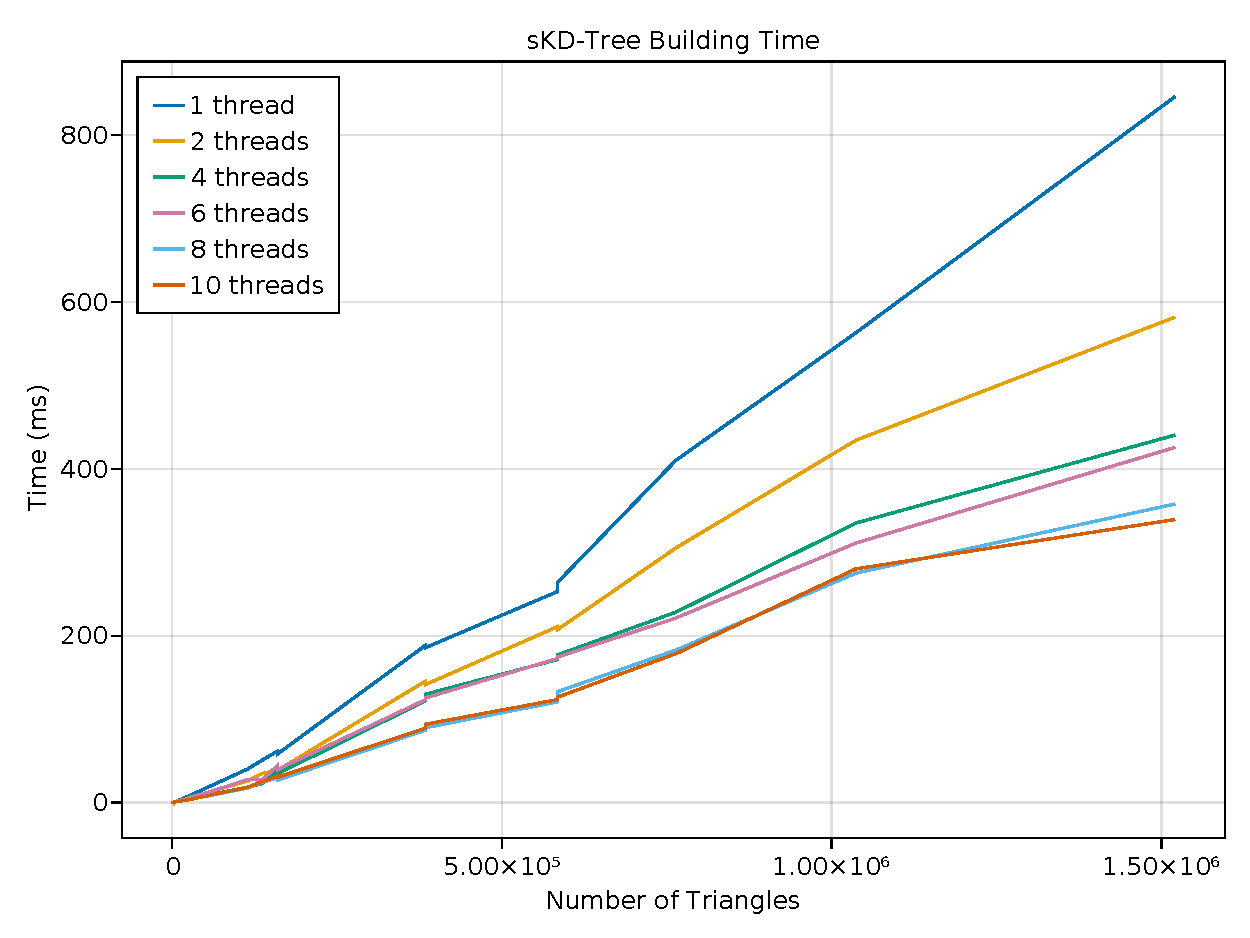
\includegraphics[width=0.6\textwidth]{build_time.pdf}
    \caption[Χρόνοι Κατασκευής του \tl{sKD-Tree}]{
        Χρόνος κατασκευής του \tl{sKD-Tree} συναρτήσει 
        του πλήθους των τριγώνων ενός πλέγματος.
    }
    \label{fig:build_time}
\end{figure}

\section{Πειράματα ανά Σενάριο}
Για κάθε ένα από τα παρακάτω σενάρια, παρουσιάζονται οι 
μετρήσεις για το κόστος αναζήτησης και το συνολικό χρόνο 
εκτέλεσης για την απάντηση ερωτημάτων απόστασης.
Στα διαγράμματα παρακάτω, γίνεται σύγκριση της επίδοσης των αλγορίθμων 
\ref{alg:queries_on_tree} και \ref{alg:search_on_two_trees}.

Το κόστος αναζήτησης υπολογίστηκε από τη μετρική κόστους 
που περιγράφεται στην ενότητα \ref{sec:cost_metric} 
μετρώντας τον αριθμό κλήσεων των ρουτινών 
\tl{\texttt{triangle\_distance()}} και \tl{\texttt{AABB\_distance()}}.

Ο συνολικός χρόνος εκτέλεσης ερωτημάτων απόστασης περιλαμβάνει 
το χρόνο προεπεξεργασίας των δεδομένων και τον χρόνο αναζήτησης.
Η προεπεξεργασία των δεδομένων είναι η κατασκευή ενός ή δύο δέντρων 
ανάλογα με τον αλγόριθμο που χρησιμοποιείται.
Οι χρόνοι που παρουσιάζονται αντιστοιχούν σε πειράματα με χρήση 
ενός, τεσσάρων και οκτώ νημάτων επεξεργασίας.

\subsection{Αεροπλάνα}

\begin{figure}[H]
    \centering
    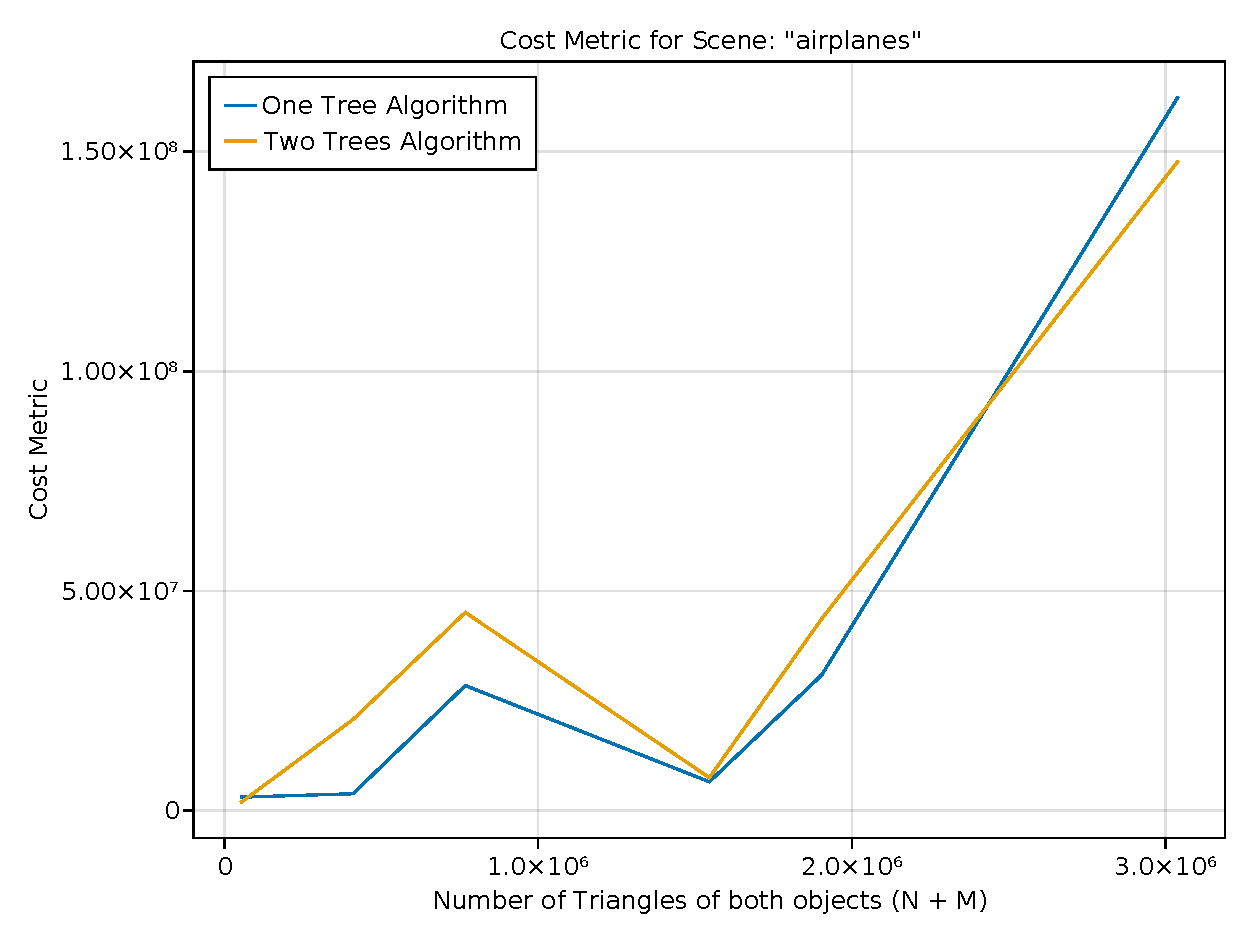
\includegraphics[width=0.6\textwidth]{cost_metric/airplanes_cost_metric.pdf}
    \caption[Κόστος Αναζήτησης για "αεροπλάνα"] {
        Κόστος αναζήτησης για τη σκηνή "αεροπλάνα" συναρτήσει 
        του μεγέθους των δύο μοντέλων.
    }
\end{figure}

\subsection{\tl{Scooby} με \tl{Stanford Bunny}}
\begin{figure}[H]
    \centering
    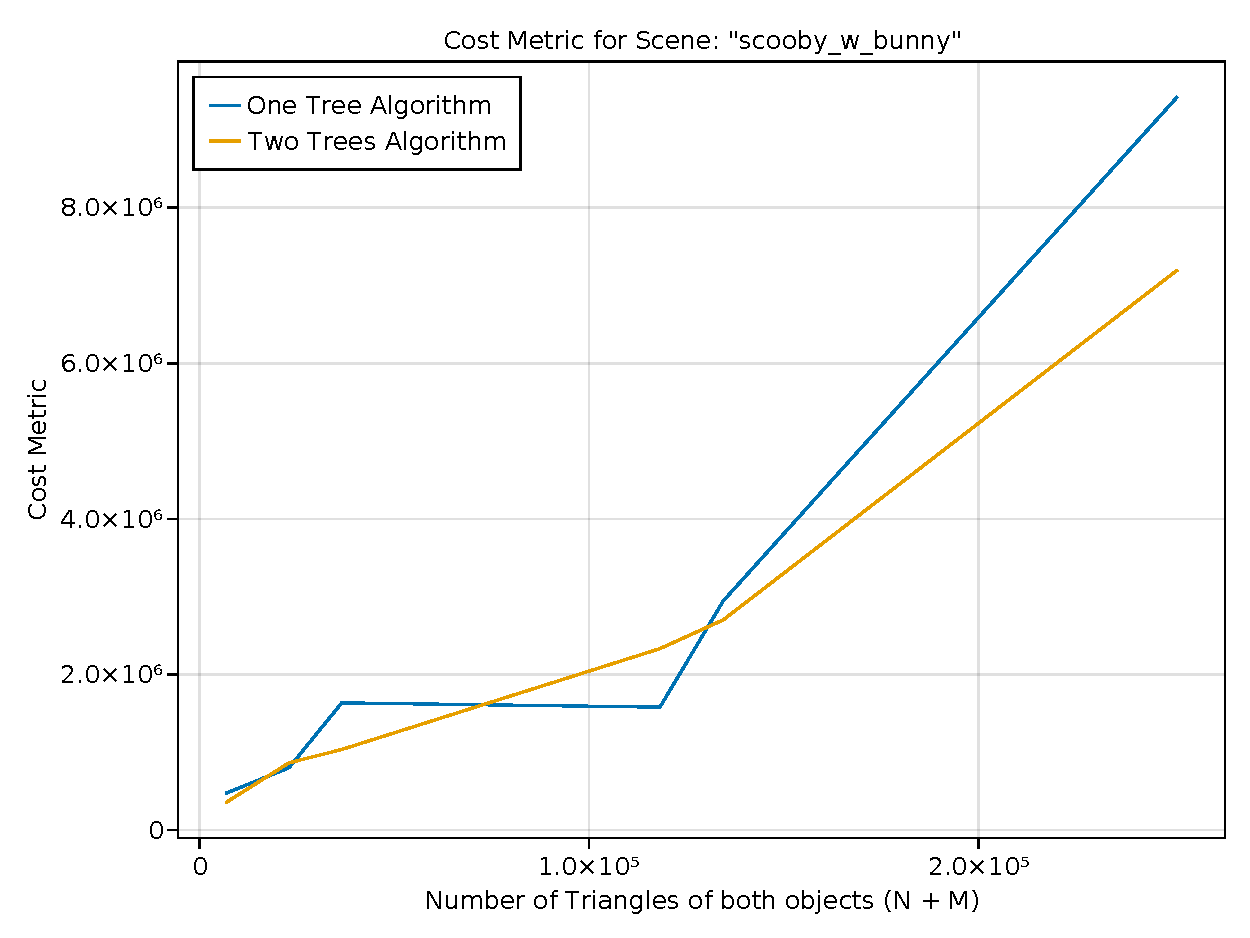
\includegraphics[width=0.6\textwidth]{cost_metric/scooby_w_bunny_cost_metric.pdf}
    \caption[Κόστος Αναζήτησης για "\tl{Scooby} με \tl{Stanford Bunny}"] {
        Κόστος αναζήτησης για τη σκηνή "\tl{Scooby} με \tl{Stanford Bunny}" συναρτήσει 
        του μεγέθους των δύο μοντέλων.
    }
\end{figure}


\subsection{Ομοαξονικοί Κύλινδροι}
\begin{figure}[H]
    \centering
    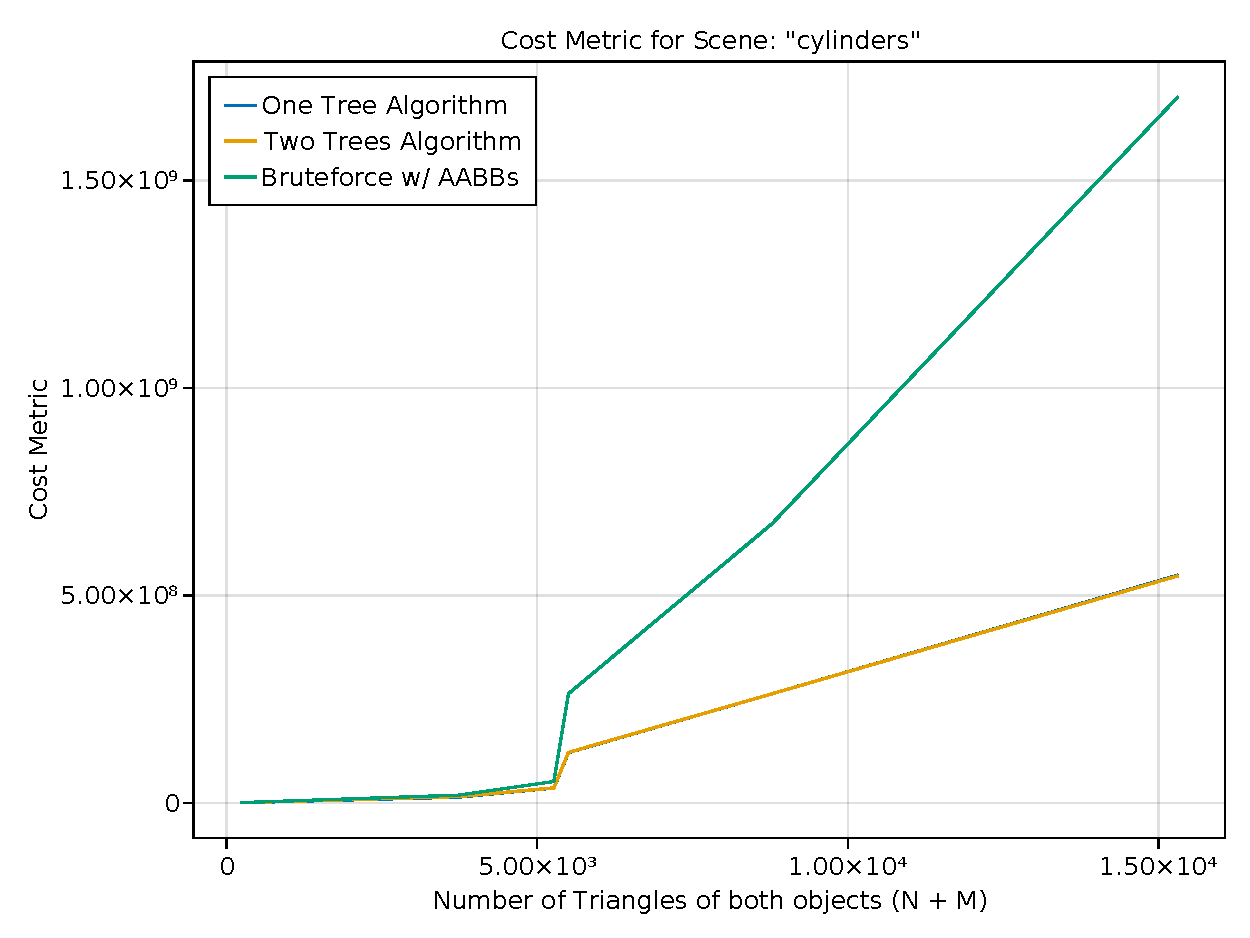
\includegraphics[width=0.6\textwidth]{cost_metric/cylinders_cost_metric.pdf}
    \caption[Κόστος Αναζήτησης για "ομοαξονικοί κύλινδροι"] {
        Κόστος αναζήτησης για τη σκηνή "ομοαξονικοί κύλινδροι" συναρτήσει 
        του μεγέθους των δύο μοντέλων.
    }
\end{figure}

\subsection{Αλυσιδωτοί Τόροι}
\begin{figure}[H]
    \centering
    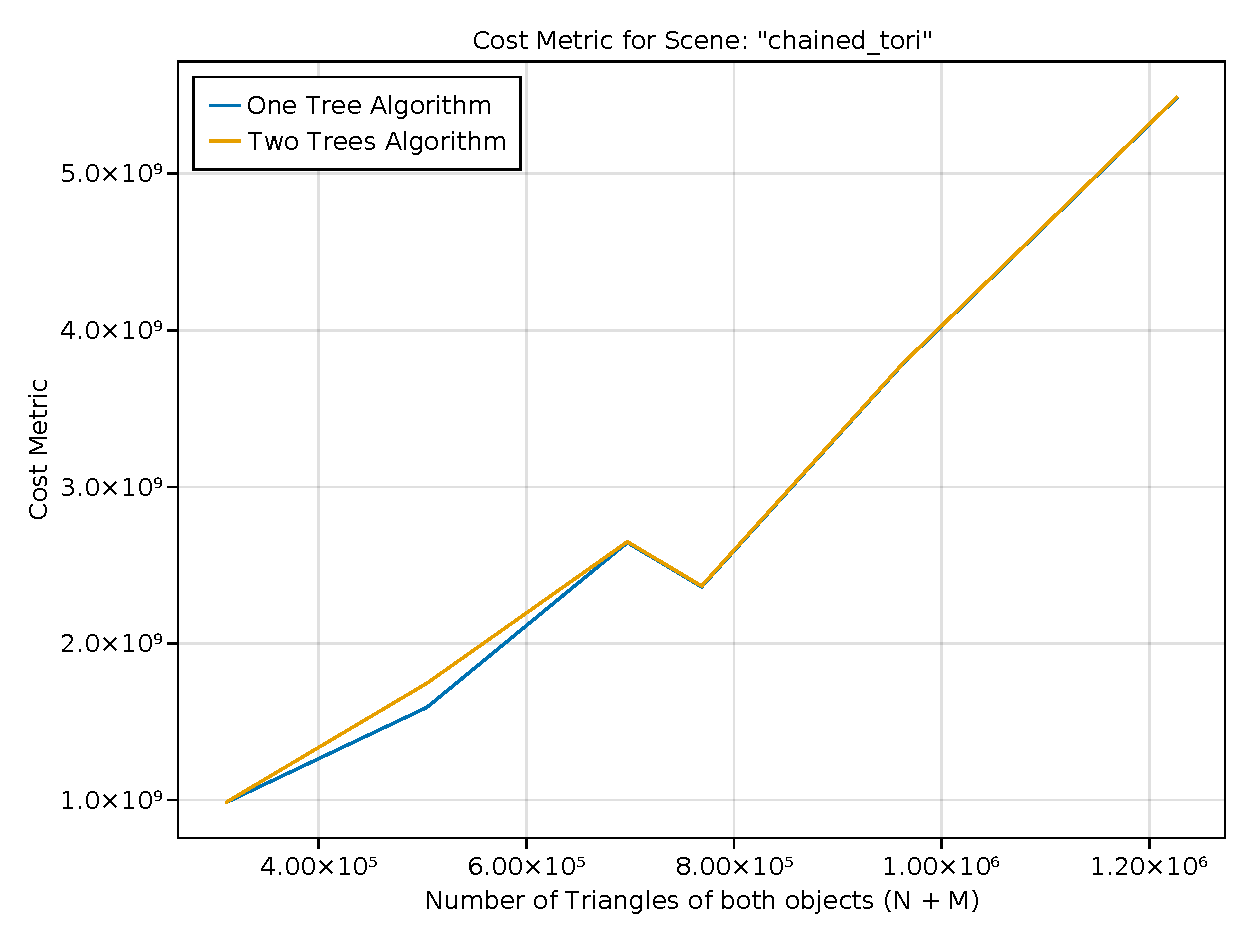
\includegraphics[width=0.6\textwidth]{cost_metric/chained_tori_cost_metric.pdf}
    \caption[Κόστος Αναζήτησης για "αλυσιδωτοί τόροι"] {
        Κόστος αναζήτησης για τη σκηνή "αλυσιδωτοί τόροι" συναρτήσει 
        του μεγέθους των δύο μοντέλων.
    }
\end{figure}

\subsection{Συγκρουόμενοι Τόροι}
\begin{figure}[H]
    \centering
    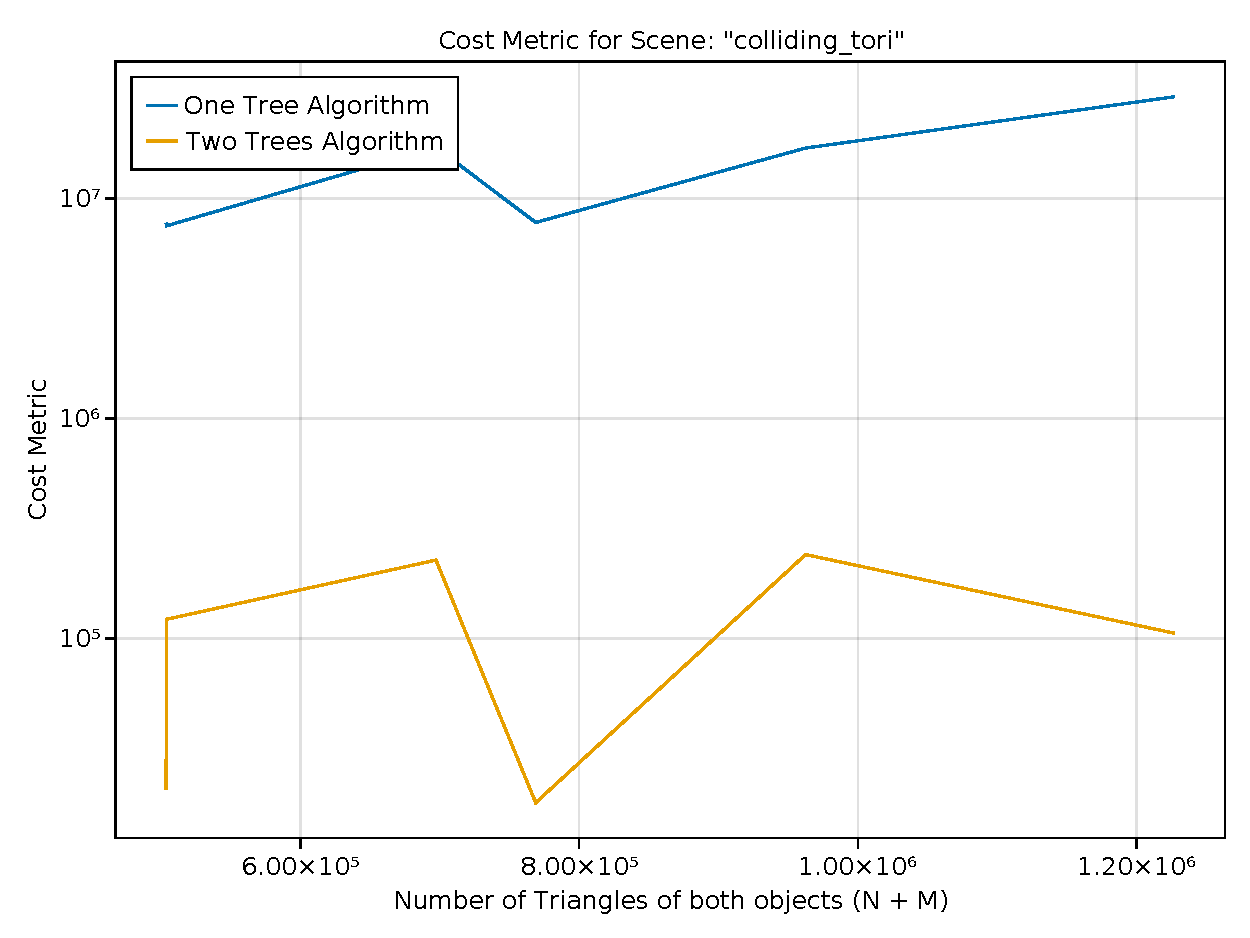
\includegraphics[width=0.6\textwidth]{cost_metric/colliding_tori_cost_metric.pdf}
    \caption[Κόστος Αναζήτησης για "συγκρουόμενοι τόροι"] {
        Κόστος αναζήτησης για τη σκηνή "συγκρουόμενοι τόροι" συναρτήσει 
        του μεγέθους των δύο μοντέλων.
    }
\end{figure}


\section{Σχέση Απόστασης - Κόστους Αναζήτησης}
Για το πείραμα αυτό επιλέχθηκαν τα αντικείμενα της σκηνής 
"\tl{Scooby} με \tl{Stanford Bunny}" με περίπου $20000$ 
και $16600$ τρίγωνα αντίστοιχα.
Αρχικά τα αντικείμενα τοποθετούνται έτσι ώστε να υπάρχει 
σύγκρουση μεταξύ τους.
Έπειτα μετακινείται το αντικείμενο \tl{Stanford Bunny} 
προς μια συγκεκριμένη κατεύθυνση ώστε να απομακρύνεται 
από το αντικείμενο \tl{Scooby}.

\begin{figure}[H]
    \centering
    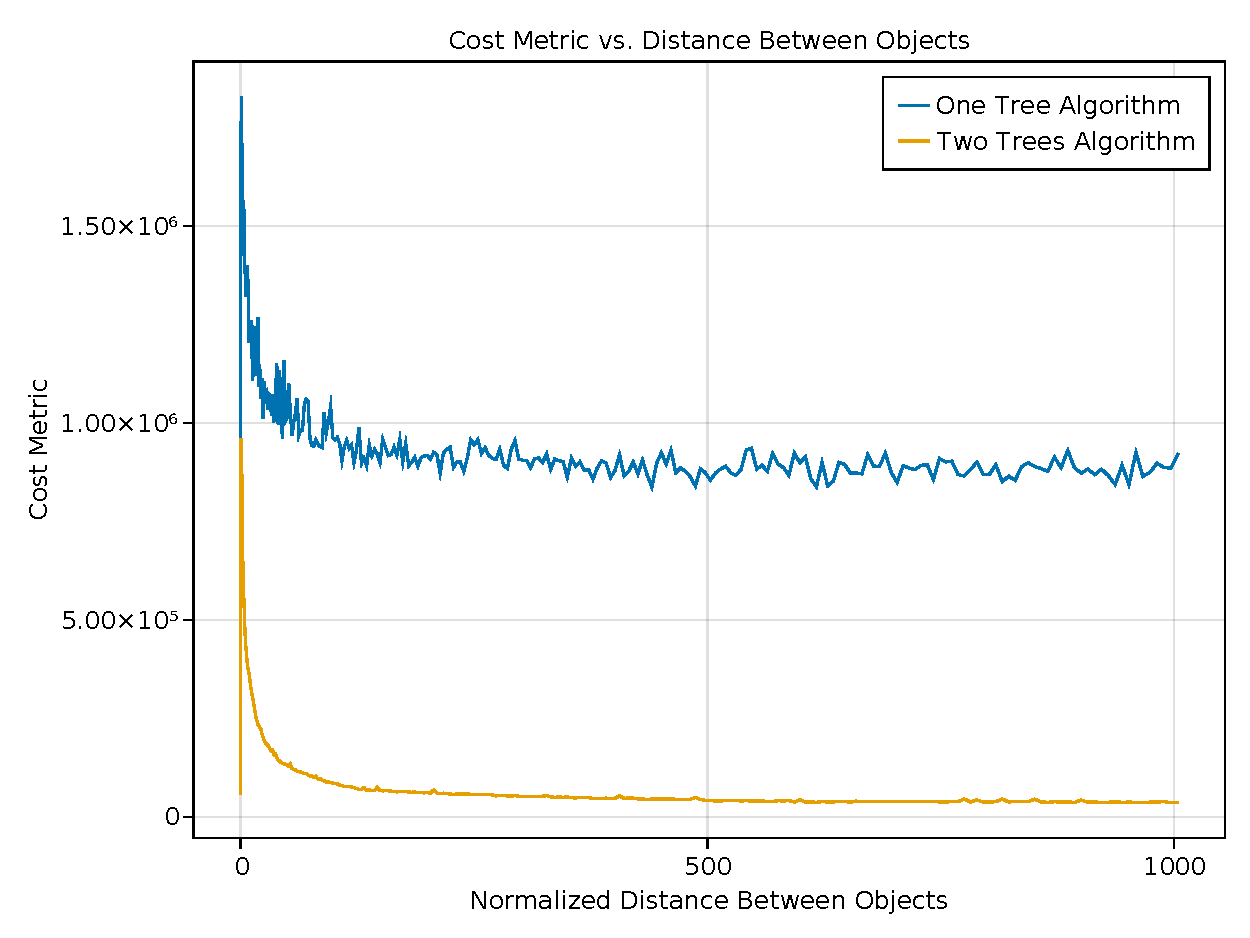
\includegraphics[width=0.6\textwidth]{cost_vs_distance.pdf}
    \caption[Κόστος Αναζήτησης Συναρτήσει της Απόστασης"] {
        Κόστος αναζήτησης συναρτήσει της απόστασης.
        Η απόσταση είναι κανονικοποιημένη και ίση με 
        $\frac{dist}{diagonal}$, όπου $dist$ η πραγματική 
        απόσταση των αντικειμένων και $diagonal$ το μήκος 
        της διαγωνίου του \tl{AABB} του \tl{Stanford Bunny}.
    }
\end{figure}


% να προσθέσω ποσοστά χρόνου αναζήτησης/κατασκευής
